\documentclass[10pt,a4paper]{article}
\usepackage[utf8]{inputenc}
\usepackage{amsmath}
\usepackage{amsfonts}
\usepackage{amssymb}
\usepackage{graphicx}
\usepackage{etoolbox,refcount}
\usepackage{multicol}

\usepackage{cite}

\newcounter{countitems}
\newcounter{nextitemizecount}
\newcommand{\setupcountitems}{%
  \stepcounter{nextitemizecount}%
  \setcounter{countitems}{0}%
  \preto\item{\stepcounter{countitems}}%
}
\makeatletter
\newcommand{\computecountitems}{%
  \edef\@currentlabel{\number\c@countitems}%
  \label{countitems@\number\numexpr\value{nextitemizecount}-1\relax}%
}
\newcommand{\nextitemizecount}{%
  \getrefnumber{countitems@\number\c@nextitemizecount}%
}
\newcommand{\previtemizecount}{%
  \getrefnumber{countitems@\number\numexpr\value{nextitemizecount}-1\relax}%
}
\makeatother    
\newenvironment{AutoMultiColItemize}{%
\ifnumcomp{\nextitemizecount}{>}{3}{\begin{multicols}{3}}{}%
\setupcountitems\begin{itemize}}%
{\end{itemize}%
\unskip\computecountitems\ifnumcomp{\previtemizecount}{>}{3}{\end{multicols}}{}}


\author{Yacine Jernite}
\title{Sequence tagging for medical problems detection}
\begin{document}

\maketitle

\section{Introduction / Reminders}

  Our ultimate goal is to identify mentions corresponding to medical problems in text and map them to UMLS CUIs. Our initial two-steps approach was to use a simple CRF for mention detection (step 1), and focus on a more elaborate method to map mentions to CUIs, or even identify mistakes of the detection (step 2).

  The reasoning behind this approach was that we felt we could make use of more interesting techniques for the second step, including leveraging MIMIC text for semi-supervised learning, and using the MRF model we developed for our ICML paper as a prior on the CUI distribution. To that end, I built a model predicting a CUI given a mention, its neighbouring words and neighbouring mentions. I first tried to do semi-supervised learning without using the MRF prior by training on MIMIC matches with different kinds of noise. I was unable to get any improvement from the MIMIC data. 

\section{Data Description / State of the Art}

  We are working on the Semeval task for analysis of clinical test. The two most recent editions of the challenge are 2014 \cite{pradhan2014semeval} and 2015 \cite{elhadad298semeval}.
  
  The 2014 edition had a training + development set of 298 notes (199 + 99) and a test set of 133 notes. In 2015, these were merged into the training + development set, and 100 notes were added as a test set (we only have access to the 298 + 133, Noemie Elhadad told us the team still had plans for a challenge involving the test set).
  
  In 2014, the challenge was divided into task 1a (identification of disorder mention span), and task 1b (mapping to UMLS, our step 2). Task 1a was evaluated for F measure, and task 1b for accuracy (recall: number of mentions correctly identified and mapped divided by number of gold mentions). In 2015, both tasks were merged, and only the global F measure was reported.

  The best result for task 1a in 2014 came from the UTH\_CCB team \cite{tang2014uth_ccb}. They achieved an F measure of 81.3 using an ensemble of CRF and Structured SVM, using UMLS, POS, cTakes output, Brown clustering and random indexing features and a \{B, I, O, DB, DI, HB, HI\} tag set. Their F measure on the global task was 71.8 (re-calculated fro their reported ``accuracy'' measure).
  
  In 2015, we only have the F measure on the global task for the fifth best team, TAKELAB \cite{glavavstakelab}. Their best development set F measure is 73.0 (with a test set F measure of 72.7). Their system is a CRF with BIO tags, post-processing for disjoint and overlapping mentions, and a set of features including SNOMED similarity and informative ngrams. The best F measure on the 100 notes of the test set (which we do not have access to) was achieved by the ezDI team with 75.7 \cite{pathak2015ezdi}, using a CRF, BIO scheme, parsing and Brown cluster features, and an SVM to re-build disjoint mentions. The UTH\_CCB team was third that year with an F measure of 73.5 on the test set \cite{xu2015uth}.
  
  AS for matching schemes, most works use some form of edit distance (TODO).
  

\section{Related Work}

For identification:
\begin{itemize}
\item Collobert et al., NLP from scratch, uses a hybrid NN-CRF model with feature embeddings for POS tagging \cite{collobert2011natural}
\item Learning character-level representations for part-of-speech tagging does the same thing with embedding of sub-word units \cite{santos2014learning}
\item Conditional random fields as recurrent neural networks formulates CRF inference as recurrent neural networks and back-propagates through the rest of the network \cite{zheng2015conditional}
\item Non-lexical neural architecture for fine-grained POS Tagging \cite{labeau2015non}
\end{itemize}

For mapping:
\begin{itemize}
\item Embedding methods for fine grained entity type classification, \cite{yogatama2015embedding} 
\end{itemize}

\section{Model description}

\subsection{CRF}
\label{CRF}

 Our baseline is a CRF with the following features (and combinations thereof):

 \begin{AutoMultiColItemize}
 \item word
 \item lemma
 \item pos (part of speech)
 \item normal
 \item word\_length
 \item prefix
 \item suffix
 \item all\_caps
 \item capitalized
 \item word\_pos (word position in the sentence)
 \item sentence\_pos (sentence position in the document)
 \item sentence\_length
 \item med\_prefix (when the word prefix matches a UMLS prefix)
 \item umls\_match\_tag\_full
 \item umls\_match\_tag\_prefix
 \item umls\_match\_tag\_acro
 \end{AutoMultiColItemize}

\paragraph{Tagging scheme}

The standard mention identification methodology consists in tagging tokens
with ‘B’ (first token of the mention), ‘I’ (other tokens of the mention) or ‘O’
labels (everything else). This reduces the problem to sequence tagging, which
can be solved linearly in the length of the sentence. For example, “the patient
suffers from a broken jaw .” will have tags O-O-O-O-O-B-I-O.
About 10\% of the mentions we are dealing with are dis-contiguous. While
those can technically be represented with a B-I-O scheme, there is a concern
that a model such as a CRF will have difficulties propagating information from
one part of a mention to another. We remedy this by adding two new labels:
‘OD’ for tokens which are within the scope of a mention but not part of the
mention itself, and ’ID’ for tokens which are part of a dis-contiguous mention.
For example, “the pain is stongest in the arm .” will have tags O-B-OD-ODOD-OD-ID-O.
About 95\% of the sentences in our data can be represented with this tagging
scheme. It fails however any time two or more mentions overlap.
It is worth noting that the vast majority of cases of overlapping mentions
in our data are of the form “A and B are C” or “A is B and C”. While any
per-token tagging scheme which covers all possible configurations would require
a prohibitively large tag set, it is easy enough to come up with one which covers
all of the aforementioned cases without making our scheme much more complex.
The idea is the following: when mentions overlap, we identify each by its
“first proper tag”. In the example “left arm and shoulder are swollen”, the
mention “left arm swollen” will be identified by “arm”, and the mention “left
shoulder swollen” by “shoulder”. We introduce a new tag ‘In’ to denote such
an identifying token (the sequence will then be labeled B-In-OD-In-OD-ID).
To make the model fully coherent however, we actually need two more tags:
‘Bn’, which acts as ‘In’ but for the first word of a mention (“elbow and wrist
broken” is labeled Bn-OD-Bn-ID), and ‘Ip’ for a token which is part of only one
of two overlapping mention, but is not the identifying token (“inflamation of
left kidney and spleen” will be labeled B-OD-In-Ip-OD-In).
This scheme uniquely defines all but 0.5\% of our sentences (it still fails in
the case of nested mentions, which exist but are quite rare).

 We reconstruct mentions from the MAP assignment of tags. The model was trained with the CRF++ package, and achieved an optimal F-measure on the development set (133 notes) of 0.78.

\subsection{New tagging models}

  We implemented two other models using TensorFlow: a neural network which predicts each tag independently(-ish) given the whole sentence (SequNN), and a hybrid neural network / CRF system (NN-CRF, the CRF potentials are the output of a neural network).

  Both have a first layer which embeds each token of the sentence into a dimension $d$ space. The embedding of a token is the sum of the embeddings of its features. So the embedding of the token {\sl{ complaining: \{lemma: complain, pos: VBG, prefix:com-, suffix, -ing, umls\_match\_tag\_full: O\}}} is:
  
  $$w_{complaining} = w_{complain} + w_{VBG} + w_{com-} + w_{-ing} + w_{O}$$

\subsubsection{SequNN}

  I tried adding various neural network architectures on top of the embedding layer, and learning the model with SGD.

  \paragraph{Convolutional layer}
  
  My current network actually consists of a single convolutional layer with window size 5, followed by a ReLU. To be perfectly clear, a convolutional window takes a window $(w_{i-2}, w_{i-1}, w_{i}, w_{i+1}, w_{i+2})$, concatenates them into a dimension $5d$ vector, then applies a linear transformation to dimension $d'$. A ReLU is then applied, followed by a linear transformation from $d'$ to the number of tags (5 currently), followed by a Soft-Max. (A picture is on its way)

  \paragraph{Bi-directional LSTM}

  I also implemented a bi-directional LSTM RNN. I couldn't get it to help however (it did worse than the ConvNet on its own, and putting the ConvNet on top of the RNN layer didn't help).

  \paragraph{Prediction targets}

  I then first replaced the marginals of output by the CRF in Section \ref{CRF} by the probabilities output by the NN. However, I could not get past an F-measure of 0.7 with this system.
  
  My next step was then to replace the tag prediction layer by a window prediction layer: instead of giving the probability of a tag, the last layer gives the probability of a tag and its left and right neighbour (125 possibilities). This got me back close to the same performance as the CRF (0.763).

\subsubsection{NN-CRF}

  \paragraph{Model}

  I also trained a neural network to output the potentials of a CRF on the tags. The current architecture is basically the same as for the per-tag (per-window) prediction: embedding layer to window 5 convolution to tanh to pair-wise potentials (5 x 5 matrices for binary potentials, and unary potentials).

  \paragraph{Learning} 
  
  The model is trained by SGD on the joint likelihood of the sequence of tags (inference is pretty fast), and back-propagating from the potentials to the NN parameters. The best F-measure obtained is about the same as the vanilla CRF. I'm hoping to play a bit with the structure and learning parameters to improve that.

\begin{figure}[h]  
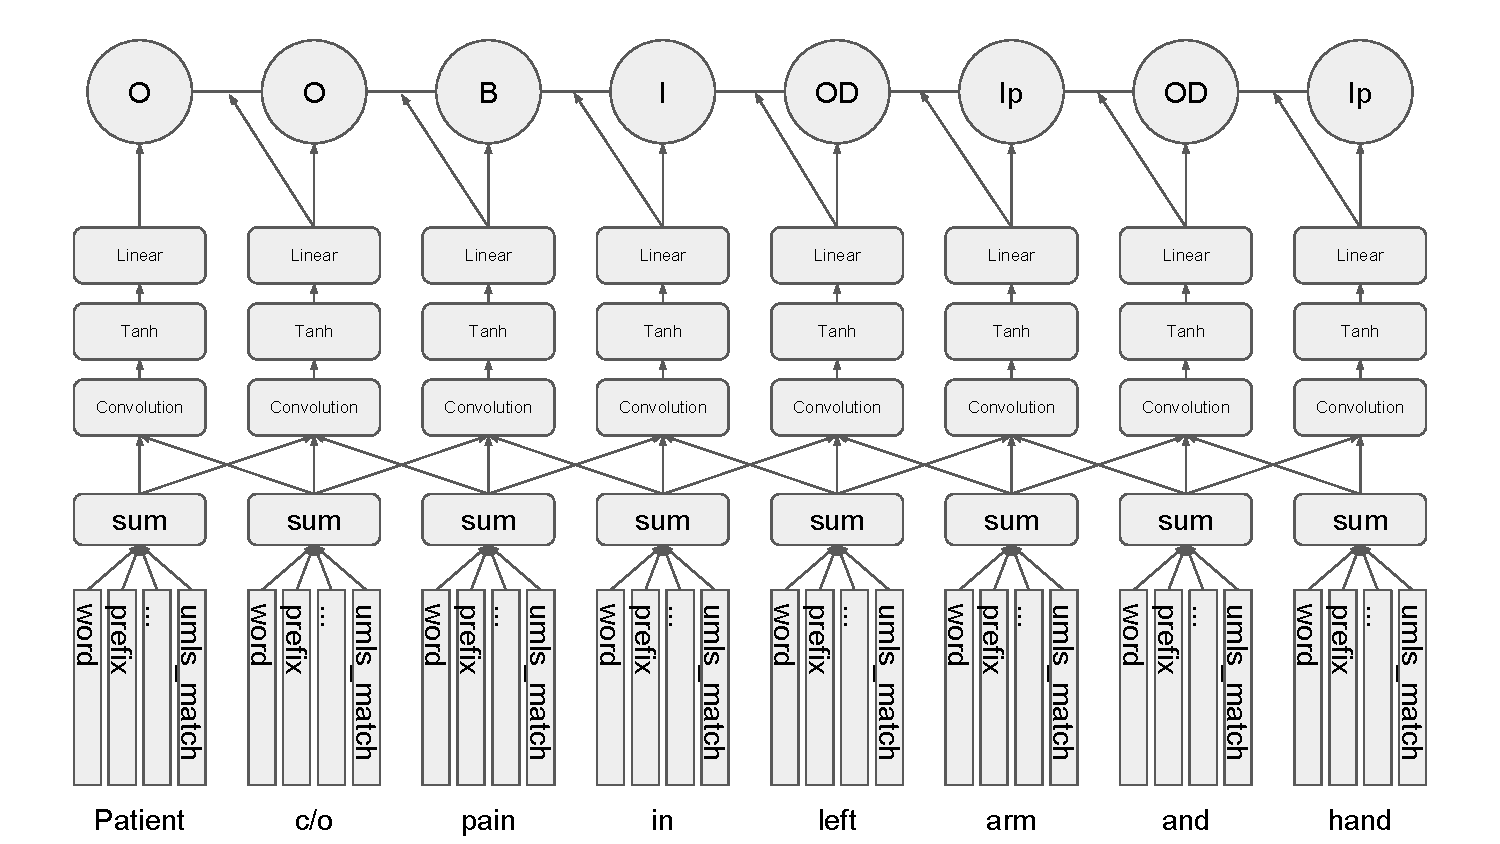
\includegraphics[width=\textwidth]{NN-CRF.pdf}
\caption{NN-CRF model}
\end{figure}

\subsubsection{Other implementation details}

I use the Adam optimizer with a learning rate of 0.02 for NN-CRF and 0.001 for SequNN, and gradient clipping. I have L1 regularization on the word, lemma and normalized word embeddings, and L2 regularization on all the embeddings. No dropout for now.

\subsection{Semi-supervised learning}

The next step is to use MIMIC to get better feature embeddings. Our idea is to learn word embeddings to predict the presence of exact matches from UMLS.

\nocite{*}
\bibliography{bibli}{}
\bibliographystyle{abbrv}

\end{document}